\documentclass{beamer}
\usepackage{../tut-slides}
\usepackage{../mathoperatorsAuD}

\usepackage{amsmath,amssymb}
\usepackage{stmaryrd}
\usepackage{enumerate}
\usepackage{csquotes}
%\usepackage[inline]{enumitem} 		%customize label
%\newcommand{\labelitemi}{\raisebox{1pt}{\scalebox{.9}{$\blacktriangleright$}}}
%\newcommand{\labelitemii}{$\vartriangleright$}
%\newcommand{\labelitemiii}{--}
\setbeamertemplate{itemize item}{\raisebox{1pt}{\scalebox{.9}{$\blacktriangleright$}}}
\setbeamertemplate{itemize subitem}{$\vartriangleright$}

\usepackage{booktabs}
\usepackage{tabularx}
\usepackage{tabu}
\newcommand*\head{\rowfont{\bfseries}}
\newcommand*{\tw}{\rowfont{\ttfamily}}
\renewcommand{\tabularxcolumn}[1]{>{\hspace{0pt}}m{#1}}

\usepackage{cancel}

%%%% EBNF-Terme %%%%
\newcommand{\wdh}[1]{\hat{\{} \ #1 \ \hat{\}}}
\newcommand{\opt}[2]{\hat{(} \ #1 \ \hat{|} \ #2 \ \hat{)}}
\newcommand{\byp}[1]{\hat{[} \ #1 \ \hat{]}}
\newcommand{\rdb}[1]{\hat{(} \ #1 \ \hat{)}}

\newcommand{\sem}[1]{\left\llbracket #1 \right\rrbracket}


\begin{document}	
	\title{Algorithmen und Datenstrukturen}
	\subtitle{Fixpunktiteration}
	\author{Eric Kunze}
	\email{eric.kunze@mailbox.tu-dresden.de}
	\city{TU Dresden}
%	\institute{Lehrstuhl für Grundlagen der Programmierung}
	\titlegraphic{
\includegraphics[width=2cm]{../TUD-white.pdf}}
	\date{}

	\maketitle


%%%%%%%%%%%%%%%%%%%%%%%%%%%%%%%%%%%%%%%%%%%%%%%%%%%%%%%%%%%%%%%%%%%%%%%%%%%%%

\begin{frame} \frametitle{Fixpunkte}
	Gegeben sei eine Funktion $f \colon \R \to \R$. 
	
	\begin{definition}
		Ein \textbf{Fixpunkt} von $f$ ist ein Punkt $x^\ast \in \R$ mit
		\begin{equation}
			f(x^\ast) = x^\ast
		\end{equation}
	\end{definition}

	\textbf{Motivation:} Lösen von Gleichungen/Gleichungssystemen
\end{frame}

\begin{frame} \frametitle{Motivation}
	Wir wollen Gleichungen der Form
	\begin{equation}
		\schlange{f}(x) = 0
	\end{equation}
	lösen. Jede solche Gleichung lässt sich leicht in Fixpunktform
	\begin{equation}
		f(x) = x
	\end{equation}
	bringen. Betrachte zum Beispiel die Gleichung
	\begin{equation}
		\schlange{f}(x) \defeq -\tfrac{1}{2} x^2 + x \overset{!}{=} 0
	\end{equation}
	mit \textit{einer} zugehöriger Fixpunktform 
	\begin{equation}
		f(x) = -\tfrac{1}{2} x^2 + 2x = x \enskip \text{.}
	\end{equation}
\end{frame}

\begin{frame} \frametitle{Ein einfaches Iterationsverfahren}
	Wollen wir nun Fixpunkte $x^\ast$ von $f$ bestimmen, so ergibt sich folgenden Möglichkeit:
	\begin{itemize}
		\item wähle \textit{geeigneten} Startpunkt $x_0 \in \R$ (in der Nähe der vermuteten Lösung)
		\item berechne 
		\begin{equation*}
				\fbox{$x_{i+1} \defeq f(x_i)$}
		\end{equation*}
	\end{itemize}
	\begin{block}{Beobachtung}
		Unter bestimmten Voraussetzungen nähert sich die Folge der $x_i$'s dem Fixpunkt $x^\ast$ an!
	\end{block}
\end{frame}

\begin{frame} \frametitle{Ein Beispiel}
	Betrachten wir wieder die Funktion $f(x) = -\tfrac{1}{2} x^2 + 2x$ und wählen als Startwert $x_0 = 0.3$.
	Dann ergeben sich folgende Werte:
	
	\begin{minipage}{\dimexpr0.3\linewidth-\fboxrule-\fboxsep}
		\footnotesize
		\begin{align*}
			x_0 &= 0.3    \\
			x_1 &= 0.555  \\
			x_2 &= 0.9559875  \\
			x_3 &= 1.45501895 \\
			x_4 &= 1.85149783  \\
			x_5 &= 1.98897355 \\
			x_6 &= 1.99993921  \\
			x_7 &= 2. \\
			x_8 &= 2. \\
			x_9 &= 2. \\
			x_{10} &= 2.
		\end{align*}
	\end{minipage}
	\begin{minipage}{\dimexpr0.7\linewidth-\fboxrule-\fboxsep}
		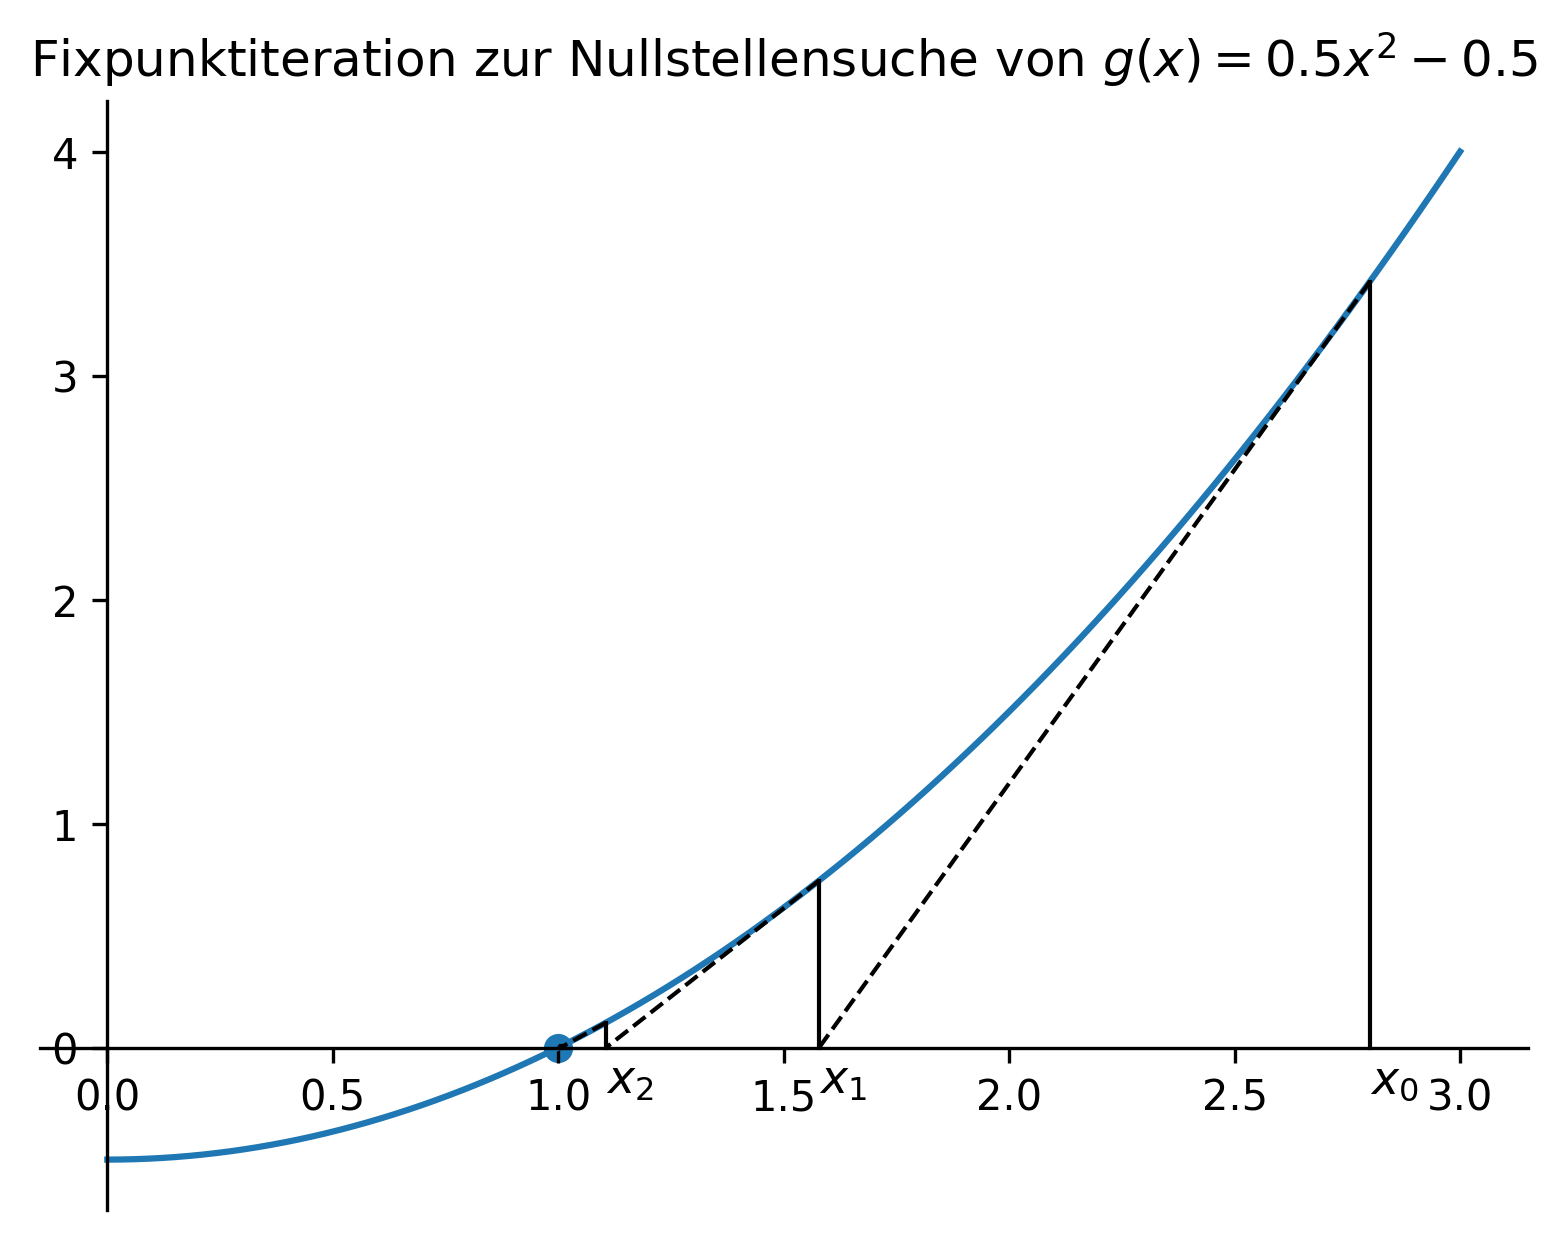
\includegraphics[width=\linewidth]{tut03_fixpunktiteration.png}
	\end{minipage}
\end{frame}


\end{document}